% !TEX root = writing_version.tex

\label{chp:simulation}
During the coarse of the master thesis an event driven molecular dynamic (EDMD) simulation code has been elaborated. The choice to use the EDMD approach is taken because interst in the actual dynamics of the system were desired. This means that simulations probing the phase space of the system instead of the dynamics, like Monte Carlo (MC) simulation schemes, are not suited.\\ 
Furthermore the discontinous potential of the hard spheres is an obstacle not easy to face in regular molecular dynamics (MD) schemes, where the Newtonian equation of motion for the particles is numerically integrated.\\
The EDMD approach on the other site actually requires these discontinuities as will be discussed in the following sections, together with some details of the program.\\

\section{Algorithm and Simulation details}
\label{sec:simulation}
%EDMD and Simulation details
In this section we will highlight the main differences to regular MD simulations, as they are the main tool to otherwise probe the dynamics of the system. Furthermore we will stick to the hard sphere example when discussing the EDMD simulations, but it can be kept in mind that the EDMD approach also allows to simulate particles with other potentials as long as the potentials are only containing step functions.\\
 
The decisive difference between EDMD simulations and regular MD schemesis that, instead of evaluating all pair and external forces on each particle and then evolving the whole system to the next time step, EDMD simulations do not have a predefined time step, but the system is evolved from one event to the next one. An event in this context is defined as the time where the next collision in the whole system takes place.\\

The event prediction algorithm is follows closely the approach proposed by Bannerman et. al \cite{Bannerman2014} which will be discussed in the next section.\\

\subsection{Event driven molecular dynamics (EDMD)}
\label{sec:EDMD}
For the prediction of events in EDMD simulations an overlap function $f_{ij}(t)$ between particles i and j is defined, where the squared quantities are used merely because they are easily accessible.\\
\begin{align}
f_{ij}(t) & \coloneqq  | \vec{r}_j(t) - \vec{r}_i(t) |^2 - \sigma^2\\
          & \; \; \, \vrule
  \begin{aligned}[t]
    \quad \text{with} \quad \vec{r}_i(t) &= \vec{r}_i(t_0) + (t-t_0) \; \vec{v}_i(t_0) \, \text{,}\\
    \Delta t \coloneqq & \; t-t_0  \, \text{,} \\ 
    \vec{v}_{ij}(t) &\coloneqq  \vec{v}_j(t) - \vec{v}_i(t) \, \text{,}\\
    \vec{r}_{ij}(t) &\coloneqq  \vec{r}_j(t) - \vec{r}_i(t) \, \text{,}\\
    \Leftrightarrow \quad \vec{r}_{ij}(t) &= \vec{r}_{ij}(t_0) + \Delta t \; \vec{v}_{ij}(t_0)
  \end{aligned}\\
f(t)  & = ( \vec{r}_{ij}(t_0) +  \Delta t \;  \vec{v}_{ij}(t_0))^2 -\sigma^2 \\
\label{eqn:overlap_f}
f(t)  & = |\vec{r}_{ij}(t_0)|^2 + \Delta t ^2 \; |\vec{v}_{ij}(t_0)|^2 - 2 \Delta t \; \vec{r}_{ij}(t_0) \cdot \vec{v}_{ij}(t_0)  -\sigma^2
\end{align}  

The overlap function has the property that it is negative for two particles being closer than their diameter, 0 for at collision and positive if neither overlapping nor touching. The calculation of the next collison thus is to calculate the roots of \autoref{eqn:overlap_f}.\\

%Solving it \todo{go to the library and take again the book to write from it the solution}
Solving for $\Delta t$ with $|\vec{r}_{ij}(t_0)|^2 \coloneqq rr $, $|\vec{v}_{ij}(t_0)|^2 \coloneqq vv $ and  $\vec{r}_{ij}(t_0) \cdot \vec{v}_{ij}(t_0) \coloneqq rv $ is rather trivial:
\begin{align}
0 &= rr + vv \; \Delta t ^2  - 2 rv \; \Delta t  -\sigma^2\\
\Leftrightarrow \quad 0 &= \Delta t ^2 - \frac{2rv}{vv} \; \Delta t + \frac{rr - \sigma^2 }{vv}\\
\Leftrightarrow \, \, \Delta t &= - \frac{rv}{vv} \pm \sqrt{\left(\frac{rv}{vv}\right)^2 - \frac{rr - \sigma^2 }{vv}}
%\label{eqn:collision_prediction_pre}
%\Leftrightarrow \, \, \Delta t &= \frac{ - rv \pm \sqrt{ (rv)^2  - vv (rr - \sigma^2 )} }{vv}\\
%\Leftrightarrow \, \, \Delta t &= \frac{rv \pm \sqrt{ (rv)^2  - vv (rr - \sigma^2 )} }{vv} \; \frac{ - rv \mp \sqrt{ (rv)^2  - vv (rr - \sigma^2 )}}{ - rv \mp \sqrt{ (rv)^2  - vv (rr - \sigma^2 )}}\\
%\label{eqn:collision_prediction}
%\Leftrightarrow \, \, \Delta t &= \frac{(rr - \sigma^2 )}{ - rv \mp \sqrt{ (rv)^2  - vv (rr - \sigma^2 )}}
\end{align}
%To circumvent a caveat when executing on a floating point machine, \autoref{eqn:collision_prediction_pre} is rewritten as in \autoref{eqn:collision_prediction}.\\ 

But a caveat when executing on a floating point machine is present as can be seen when considering which solution is of interest. As for a possible collision it is necessary that the two particles move towards each other we can conclude that the scalar product is required to be negative $rv<0$, because otherwise the particles are already moving away from each other.\\ 

Also the quadratic formula has two solutions, corresponding to the entry and the exit of the overlap. Because the entry has to be prior to the exit, we further conclude that interest lies on the smaller solution that is:
\begin{align}
\label{eqn:collision_prediction_pre}
\Delta t &= \frac{ - rv - \sqrt{ (rv)^2  - vv (rr - \sigma^2 )} }{vv}
\end{align}
Now for the case where the distance of the spheres is already close to the diameter of the spheres we find $(rv)^2 \gg (rr-\sigma^2)$, which results in a cancelation of two large numbers leaving a small number. Floating point number operations are inherently bad suited because they tend to large inaccuracy in this case. Rewriting \autoref{eqn:collision_prediction_pre} by making use of the third binomial formula \todo{look if this is fine to write.} leads to:
\begin{align}
\label{eqn:collision_prediction}
\Delta t &= \frac{(rr - \sigma^2 )}{ - rv + \sqrt{ (rv)^2  - vv (rr - \sigma^2 )}}
\end{align}
Comparably \autoref{eqn:collision_prediction} does not contain a cancelation of the type seen before and such is better suited for the use in a computer simulation. \todo{cite Goldberg '91}\\

%The algorithm proposed by Bannermann\cite{Bannerman2014} works by differentiating 4 cases:
%\begin{description}
%\item[First,] \hfill \\ if $rv>0$ the particles move away from each other leading to a collision time of $\Delta t = \infty$.
%\item[Second,]\hfill \\ if $rr<\sigma^2$ an overlapis present resulting in an immediate collision time of $\Delta t = 0$
%\item[Third,] \hfill \\ if $(rv)^2  - vv (rr - \sigma^2 ) \leq 0 $ the two particles miss each other, including touching without momentum transfer, resulting in a collision time of $\Delta t = \infty$
%\item[Fourth,] \hfill \\ if none of the before is given the particles collide and $\Delta t$ is calculated by \autoref{eqn:collision_prediction}.
%\end{description}

The event prediction algorithm proposed by Bannermann\cite{Bannerman2014} works by differentiating 4 cases:
\begin{enumerate}
\item If $rv>0$ the particles move away from each other leading to a collision time of $\Delta t = \infty$.
\item If $rr<\sigma^2$ an overlap is present resulting in an immediate collision time of $\Delta t = 0$
\item If $(rv)^2  - vv (rr - \sigma^2 ) \leq 0 $ the two particles miss each other, including touching without momentum transfer, resulting in a collision time of $\Delta t = \infty$
\item If none of the before is given the particles collide and $\Delta t$ is calculated by \autoref{eqn:collision_prediction}.
\end{enumerate}

All collision times for a particle are then stored in a queue sorted by event time called particle event list (PEL). From the PEL the first entry is then passed to the global FEL.\\
This procedure initally takes place for all particles to set up the system and later on for particles involved in an event after its execution.\\ 

As will be discussed in \autoref{sec:implemetation} some widely used measures like reducing redundant calculations or implementing a cell system to reach $\mathcal{O}(N)$ computation timehave been implemented.\\

A further detail to take care of is the possibility of scheduled events which have bcome invalid due to a earlier collision of the one of the particles. This is handeled by assigning an interaction count to each particle and then store this at precalculation time with the event. When the event comes up, and the interaction count of one of the particles has increased in the meantime, the event is said to be invalidated. Depending on which particle had an event in the meantime the invalidation either causes no action or a recalculation of new events.\\  

\subsection{Details of the Implementation} 
\label{sec:implemetation}
%Add Details of for example FEL, and backupevent handling, double time precision, reset sim
As the simulation code is based on an earlier Monte Carlo Code for hard spheres a complete walk through the whole progam would become quite extensive. Such we will focus on key points to understand the details of the simulation.\\

\subsubsection{\textit{Event} struct}
\label{sec:event_struct}
We start with the basic \textit{Event} struct which includes 6 entries as shown in \autoref{tab:event_entries}.
\begin{table}[h!]
\centering
\begin{tabular}{c|c}
\textbf{Datatype} & \textbf{Name of entry}\\ \hline
(timeType) & time \\
(int) & event\_type \\
(particle*)  & particle \\
(void*) & partner \\
(int) & particle\_count \\
(int) & partner\_count \\
\end{tabular}
\caption{Content of the \textit{Event} struct.}
\label{tab:event_entries}
\end{table}
The type of \textit{time} (timeType) is usually set to double. The \textit{time} variable itself represents the time for when the event is scheduled.\\ 
The \textit{event\_type} variable is either set to 0 or 1 and indicates if the event is a cell transfer or a collision of two particles.\\
The \textit{particle} variable is a pointer to the particle for which the event has been pre calculated, while the \textit{partner} variable is set to be a void pointer. Such it is possible to either interpret it as a particle pointer for the collision type event or as an interger pointer to the index in the current cells' neighbours list for transfer events.\\
In the last two rows the interaction counts for particle and partner are listed as well. As the destination cell in a transfer event does not require an interaction count, the \textit{partner\_count} variable is only used for collision events.\\

The \textit{event} struct is used for all events throughout the simulation. For read and write operations with the HDF5 file format, the struct \textit{event\_data} is available which uses only indexes instead of pointers.\\

\subsubsection{\textit{Particle} class}
\label{sec:particle_class}
The \textit{Particle} class is comparably to the one from the MC code basis. Its MC related variables have been removed and additional key variables and concepts will be discussed in the following:\\

First a vector storing events called \textit{backupEvent} has been added to make it possible to store events from the pre calculation for the case of the first event being invalidated. The idea of reusing events is discussed in many publications, for example that the memory cost increases onyl moderately with more backup events while the speedup does not increase much for more than two stored events \cite{Bannerman2011}. It also has been argued that the added complexity can not account for the increase in efficency\cite{DONEV2005}.\\ 
Eventhough in the own simulations a decrease in calculation time of more than 10\% was observed and the cost of complexity was seen as moderate. The difference might be explained by the fact that the systems under consideration in this thesis have a rather large particle density, leading to more invalid collsions.\\

In the context of reusing pre calculated results, it should also be mentioned that after a cell transfer the recalculation of events can be restricted to partner particles only in the new neighbouring cells, leading to only 1/3 of the calculation time in this case. But as mentioned systems under consideration are mostly rather dense and such the number of transfers is often at below 5\%. Thus the increase in efficency was assumed to be to costly on the complexity side, and not implemented. Eventhough for sparse systems, it might make sense to include an \textit{updatePEl} routine.\\


Also key differences to the former MC Particle type are the variables \textit{total\_interactions} and \textit{particle\_delayed\_time}. The first is the variable for book keeping of interactions, while the second represents the event driven character of the simulation. Because each particle only moves on purely ballistic trajectories until an event occurs, it is not necessary to keep all particle positions and velocities synchronized in time. Quite on the contrary it would mean executing extra operations together with summing rounding errors by each floating point operation.\\

Because sometimes it is desired to have the whole configuration at one point of time, the \textit{transferToTime()} function of the particle provides the possibility to take the particle into the present. This is necessary soon as measurements are performed on the system, including snapshots.\\

As mentioned before the system behaves chaotic even under slightest changes like a rounding error from an extra floating point operation. A result of this is that measuring at different rates during a simulation changes the simulation trajectory quite a bit. It has been observed that such a system may keep close to the undisturbed trajectory for about 50-100 events/particle. As it is of desire to measure quantities and take snapshots without disturbing the simulation, the simulation program makes employs copies of the configuration being costly in terms of memory but making simulation resets or higher sampling rates at interesting points possible within a defined trajectory.\\ 

The structure is as follows: The first copy is rewritten with an image of the working configuration just before any measurement. The working trajectory iteself is then disturbed by the measurement, and afterwards replaced with its state before the measurement from the backup configuration.\\
The second copy actually includes the full simulation state, while the first only includes the particle cofiguration. This second one might be used to save a state during the simulation and reset to just the same point at any later time.\\


\subsubsection{The \textit{Box} class}
\label{sec:box_class}
The box of the simulation stayed mostly the same as in the previous MC code. One chanege is the array \textit{neighbours\_lookup} which has been added. It contains the indices for the cells' \textit{neighbours} array pointing to cells that share their surface. It is used to identify which cell a particle has to be transfered to during a cell transfer event.\\

Furthermore the \textit{Update} routine now takes care of all quantities depening on the length of the box, making the \textit{rescale} routine a simple rescaling of the edge lengths with an additional \textit{Update} command.\\

\subsubsection{The \textit{Scheduler} class}
\label{sec:scheduler_class}
While the afore mentioned parts of the program are necessary for the EDMD program, the \textit{Scheduler} class contains the most distinct parts of the program. It keeps track of all events to come, predicts new events and orchestrates the execution of the events. The essential functions are discussed in the following subsections while some basic properties are shortly highlighted here.\\

First of all the \textit{Scheduler} holds the Future event list (FEL) in which at least one event per particle is stored. As discussed within \autoref{sec:particle_class} the simulation is capable of saving the complete state of a trajectory, including all pre calculated events. For this purpose an array of \textit{Events} is available.\\
Furthermore the \textit{Scheduler} includes the \textit{gloabl\_time}.\\
Important for the efficency is the pre allocation of all arrays used within the prediction calculations, as the number of executions for the collision prediction routine is about $\frac{30}{\text{particle} \cdot \text{step}}$ accounting to a few billion function calls during a small simulation.\\

\subsubsection{\quad \textit{Scheduler::predictTransfer()}}
As the name suggests this function predicts the next cell transfer of a particle due to its movement. For this it calculates the position of the particle at global time, which for a valid state of the simulation always lies within its cell. By transforming the momentary position of the particle from the global coordinate system to the coordinate system of the cell and taking into account the periodic boundary conditions, we can write for each dimension $i$ the equations
\begin{align}
t_{i1}=-\frac{r_i}{v_i} \quad \text{and} \quad t_{i2}=\frac{l_i-r_i}{v_i}
\end{align}
which describe the times when the particle pierces the cell's left and right boundaries. A negative time corresponds in this case to a boundary crossing in the past, a time comparable to 0 means that the particle is on the edge of its cell and a positive time means that the boundary crossing lies in the future. By going through the different possible cases for $t_1$ and $t_2$ we find the resulting next crossing time for each case as shown in \autoref{tab:crossing_times}.
\begin{table}[h]
\centering
\begin{tabular}{c|c||c|c}
$t_1$ & $t_2$ & Result & Case \\ \hline
> & > & invalid & - \\ \hline
> & = & $t_{\text{crossing}} = t_1$ & 0 \\ \hline
> & < & $t_{\text{crossing}} = t_1$ & 1 \\ \hline
= & > & $t_{\text{crossing}} = t_2$ & 2\\ \hline
= & = & invalid & - \\ \hline
= & < & $t_{\text{crossing}} = t_1$ & 3 \\ \hline
< & > & $t_{\text{crossing}} = t_2$ & 4 \\ \hline
< & = & $t_{\text{crossing}} = t_2$ & 5\\ \hline
< & < & invalid & - \\ \hline
\end{tabular}
\caption{Possible results for left and right crossing time with resulting choice of next crossing time. >, = and < are to be read as for example $t_1 > 0$. The case indicates the case number within the actual simulation.}
\label{tab:crossing_times}
\end{table}

By collecting the next crossing times for each dimension and taking the minimum of these times the exit time of the particle from its cell is determined.\\

The return value of the routine is an \textit{Event} where the partner is given as an address to the box' \textit{neighbours\_lookup}. The index lies between 0 and 5, corresponding to the 6 possible neigbhour cells sharing a surface with the current cell of the particle. Each valid case represents a distinct neigbour cell and the index within the cells \textit{neighbours} array is clearly defined by the cell setup routines and is shown in \autoref{tab:cell_neighbour_index}. 

\begin{table}[h]
\centering
\begin{tabular}{c|c|c|c}
dimension & boundary & case & index \\ \hline
x & front & 0 & 12 \\
 & back & 1 & 13 \\ \hline
y & front & 2 & 10 \\
 & back & 3 & 15 \\ \hline
z & front & 4 & 4 \\
 & back & 5 & 21 \\
\end{tabular}
\caption{Overview of the cells' \textit{neighbours} indices directly sharing a surface for 3 dimensions. As the indices hardly follow any simple pattern they are explicitly noted at this point. Obviously the cell consists of a front and a back boundary in each dimension. The corresponding case matches the one from \autoref{tab:crossing_times}.}
\label{tab:cell_neighbour_index}
\end{table}
\FloatBarrier

\subsubsection{\quad \textit{Scheduler::predictCollision()}}
The prediction of collision times has already been discussed in \autoref{sec:EDMD}. The implementation in the program first calculates all necessary scalar products while accounting for the periodic boundary conditions, and in a second step returns the collision time depending on the case at hand.\\

The presented algorithm is only valid for single sized particles. If polydisperse systems are supposed to be considered the algorithm has to be adjusted. \todo{mayhap do it in the appendix?}\\

As this routine is executed through out the simulation very often it has been tried to optimize its efficency multiple times. For example calculating only necessary results for the next case differentation has been implemented but no significant increase in efficency was recognized and for better readability the prior version has been reestablished. In either case if an optimized way of calculating the results is found it might be useful to use them.\todo{<-- Not really nice}\\    

\subsubsection{\quad \textit{Scheduler::setupFEL()}}
This routine fill the FEL of the simulation. For this purpose it iterates through all particles and calls \textit{setupPEL} for each of them. The PEL in turn is set up by predicting the next cell transfer as well as the next collisions with all particles within the $3^d$ cells directly surrounding the particle. From all predicted events only such with finite times are then written to the \textit{backupEvents} vector corresponding to the PEL of the particle.\\
For the FEL only the top event of each particle is then used. Because other events from the PEL are able to move on to the FEL ounce written to the FEL an event has to be erased from the PEL.\\

\subsubsection{\quad \textit{Scheduler::executeTransfer()}}
The execution of a transfer event is accomplishd by the event particles \textit{MoveBetweenCells()} routine. The departure cell is taken as the event particles own cell. While the event partner holds the information which of the cell neighbours is the destination cell.\\

\subsubsection{\quad \textit{Scheduler::executeCollision()}}
The outcome of a collision between particle 1 and 2 with corresponding position and velocity can be derived by momentum and energy conervation \todo{cite some textbook, or better jsut write down the calculation} too be 
\begin{align}
\label{eqn:collision_result}
\vec{v}_1^{\,'} = \vec{v}_1 + \left( \frac{\vec{r} \cdot \vec{v} }{\vec{r} \cdot \vec{r}} \right) \vec{r}_{12}
\end{align}
While \autoref{eqn:collision_result} is not directly depending on the radius, an indirect dependence  by the collision time and configuration at which \autoref{eqn:collision_result} is evaluated persists.
 
\subsubsection{\quad \textit{Scheduler::executeEvent()}}
The execution of an event works in multiple steps. At first the topmost \textit{Event} is copied from the FEL where it is deleted. Next the validity of the interaction counts of both particle (\textit{cond1}) and its partner (\textit{cond2}) are evaluated. The validation is nothing else than a comparison of the interaction counts when the event was scheduled with the present interaction counts. As the conditions are used in the following flow statements they are stored as boolean type. Furthermore in the case of a transfer event the validation of the partner is not necessary but only for better readability performed.\\
It follows a distinction between 5 cases which are given by:
\begin{description}
\item[Valid transfer (\textit{event\_type}==0 and \textit{cond1}) ] \hfill \\ The transfer is executed, the global time is evolved to the event time and the particles PEL is rebuilt and its next event pushed to the FEL.
\item[Valid collision (\textit{event\_type}==1 and \textit{cond1} and \textit{cond2}) ]\hfill \\ The collision is executed, the global time is evolved to the event time and for both particpating particles new PEL's are built and each top event is pushed to the FEL.
\item[Invalid transfer (\textit{event\_type}==0 and not \textit{cond1})] \hfill \\ The particle must have had an interaction previously where a new event for it was scheduled, thus no action is taken.
\item[Invalid collision due to particle (\textit{event\_type}==1 and not \textit{cond1})] \hfill \\  The particle must have had an interaction previously where a new event for it was scheduled, thus no action is taken as for the above.
\item[Invalid collision due to partner (\textit{event\_type}==1 and not \textit{cond2})] \hfill \\  Only the partner had an interaction previously where a new event for it was scheduled, thus a new event for the particle is required. As the particle had no further interactions, the \textit{backupEvents} are still valid and its first entry is pushed into the FEL. In case no backupEvents are stored the PEL is rebuilt and its first entry pushed to the FEL instead.
\end{description}
The order of the cases might be exchanged, except for the last two. This is because the last one assumes \textit{cond1} to be true, which is guaranteed by the case before.\\

Furthermore the routine counts the number of each case, to monitor numbers of collisions, transfers and invalidated cases by type. This is not required by the simulation but can be helpful for understanding the system and simulation.\\




\section{Measurement quantities}
\label{sec:cluster_quantities}
list quantities and their use etc.

\subsection{Mean squared displacement}
\label{sec:MSD}
-Averaged or as distribution\\
-Reuqired for diffusion\\

\subsection{Radial distribution fucntion}
\label{sec:RDF}
-Well show an RDF?

\subsection{Largest Cluster}
\label{sec:lc}
- Non local\\
- large in case of nucleation\\
- requires almost no memory\\

\subsection{Cluster size distribution}
\label{sec:pnt}
- Non local\\
- requires more memory still not as much as for example particle positions\\
- 

\subsection{Cluster positions and numbers}
\label{sec:cluster_position}
- not done\\
- local as single clusters can be named and followed from formation to melting or final growth\\
- Much more information as locallity can be archieved.\\


\subsection{Tensor of Gyration}
\label{sec:ToG}
-Only done for largest cluster of size larger than some threshold\\
-How to extract the eigenvalues l1,l2,l3\\
-Radius of Gyration\\
-Anisotropy\\
-Asphericity\\

\subsection{Individual cluster tracking}
\label{sec:tracking}
To follow trajectories of single metastable clusters within the fluid is of interst as mean lifetimes and other quantities of these fluctuations can be measured with it. Because the clusters themself form out of the liquid and are not numbered and easily distinguisable as the particles are in the simulation, they have to be identified for each measurement step. They are mostly characterized by the participating particles and their center of mass position, of which the later one is easier for comparisons. An algorithm based on a maximum of expected movement from one time step to the other yields reasonable results as can be seen in \autoref{fig:cluster_tracking_example}.


\begin{figure}[h]
\centering
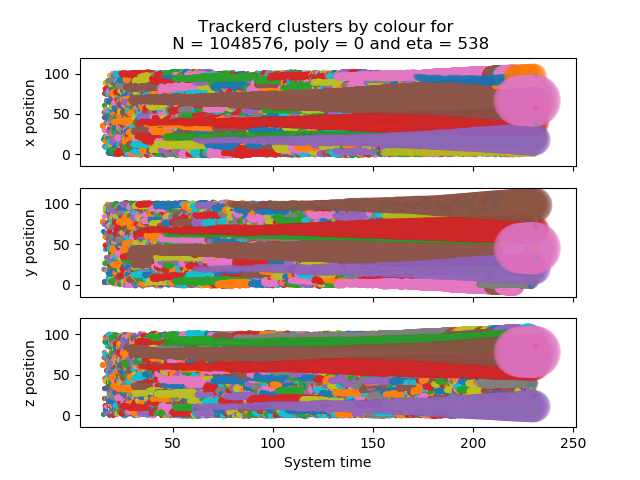
\includegraphics[width=0.7 \linewidth]{cluster_tracking_example.png}
\caption{Example results of cluster tracking algorithm in a polydisperse simulation. The three plots are the projections of the box onto the three spatial dimensions over time. Further each cluster is given a color which does not change over time. Such we can see for example that two clusters mingling in one projection are actually some distance apart from each other.}
\label{fig:cluster_tracking_example}
\end{figure}

\begin{figure}[h]
\centering
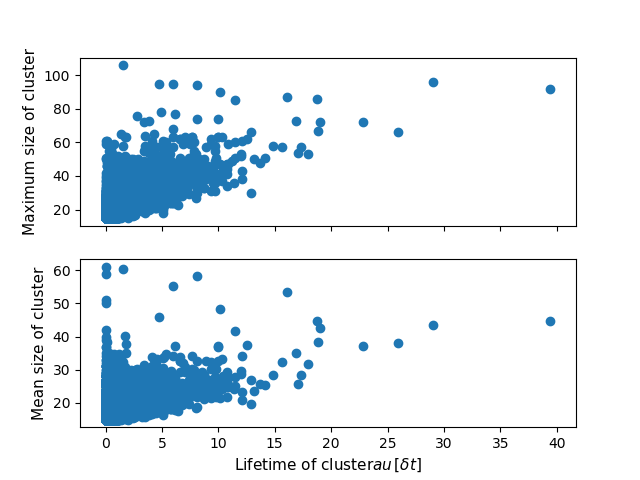
\includegraphics[width=0.7 \linewidth]{cluster_tracking_lifetime.png}
\caption{Example of lifetime depending on mean or maximum size of the metastable cluster.}
\label{fig:lifetime}
\end{figure}



\section{Probe of simulation code}
\label{sec:probe}
To probe the simulation dynamics we measuremed the longtime diffusion constant and the radial distribution function of the stable hard sphere liquid, as there are many measurements available in the literature to compare with.

\subsection{Diffusive behaviour}
\label{sec:diffusion_probe}
The diffusive behaviour of particles in a liquid usually can be three sepearted in thee distinct parts. First the short time diffusion which can be understood as the random movement of the particles within their momentary cage within the fluid. Second a sub diffusive phase in which the particles are repelled for the first time by their nearest neighbours. And third the long time diffusion to describe the random propagation of the particle through the fluid over time.\\
   
As the ballistic hard sphere system enters into the long time diffusion almost at ounce only this is really measureable. By assuming a diffusive process we have the expectaion that the average mean squared displacement (MSD) of a particle can be well described by 
\begin{align}
\label{eqn:diffusion}
\langle x^2 \rangle(t) = 2 \, d \, D \, t  \, \text{,}
\end{align}
where $\langle x^2 \rangle$ is the expectation value of the MSD, $d$ the number of spatial dimensions, $D$ the characteristic diffusion constant, and $t$ the time by which the system has evolved.\\

By measuring $\langle x^2 \rangle (t)$ and making a linear regression to the data points we can find the Diffusion constant $D$.

To probe the simulation code, systems as characterized in \autoref{tab:system_diffusion} have been used. The equilibration phase has been carried out up to $\eta_f = 50\%$ at the final volume fraction while above $\eta_f =  50\% $ an inital volume fraction of $\eta_i = 45\%$ has been used to obtain a fluid rather than a solid after the equilibration phase. As the measurement stretches into the metastable regime, it has also been necessary to check for nucleation events which were not present during the measurements.\\

The resulting diffusion constants depending on the fluid volume fraction are shown in \autoref{fig:diffusion_const} alongside values obtained from the literature, for a similar system.\\

\begin{figure}[h]
\centering
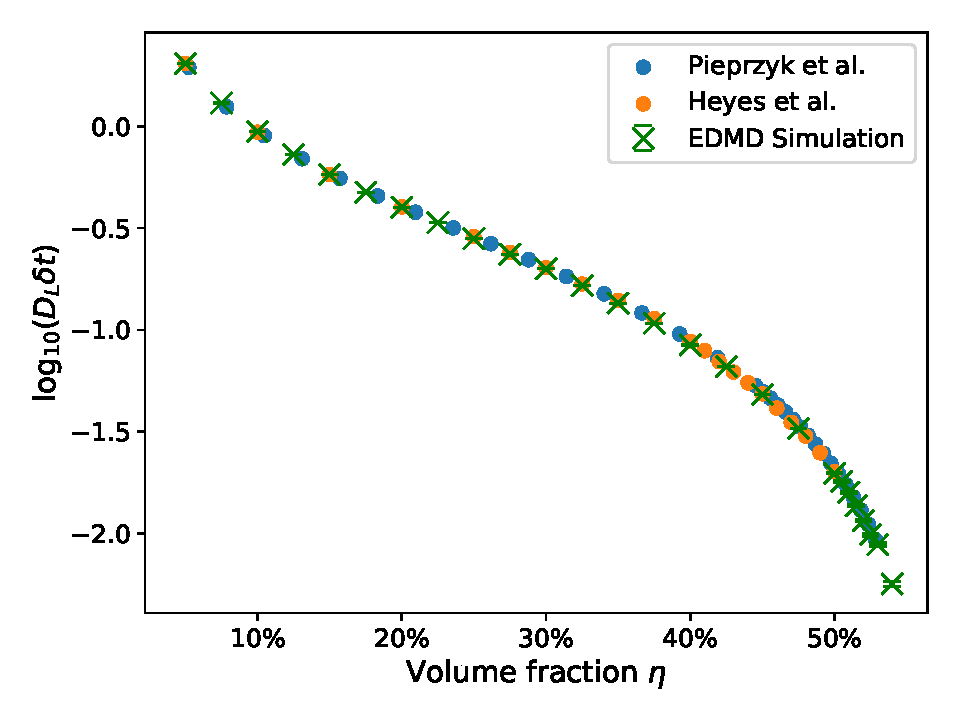
\includegraphics[width=0.7 \linewidth]{diffusion_probe.pdf}
\caption{Logarithmic long time diffusion constant of the hard sphere liquid as measured in the own simulations as well as measurements from the literature. \todo{cite the people.}}
\label{fig:diffusion_const}
\end{figure}

As it can be seen the EDMD simulation is very well capable of reproducing the diffusion constant for the hard sphere liquid, and such we expect the dynamics of it to accurately represent the purely ballistic hard sphere system.\\


\begin{table}[h]
\centering
\begin{tabular}{c|c}
Parameter & Value \\ \hline
N & 16384 \\
eq\_steps/particle & 5000 \\
pr\_steps/particle & 20000 \\
$\eta_i$ & 5\% ... 50 \% \\
$\eta_f$ & 5\% ... 54 \% \\
\end{tabular}
\caption{Input parameters of diffusion test systems.}
\label{tab:system_diffusion}
\end{table}





\subsection{Radial distribution function}
\label{sec:RDF_prob}
A further well known quantity for the hard sphere system is the radial distribution function. As a theoretical prediction the Percus-Yevick approximation can be used to compare with, also it would be possible to compare with Monte Carlo simulations of the hard sphere system. In \autoref{fig:rdf_overview} an overview for a range of volume fractions is shown from the same simulations used in \autoref{sec:diffusion_probe}. Clearly visible is that no particles enter within the diameter of the spheres. Further for higher volume fractions the liquid shells become very well visible. At very high volume fraction we also find that  new peak arises below $r = 2 \sigma$.
\begin{figure}[h]
\centering
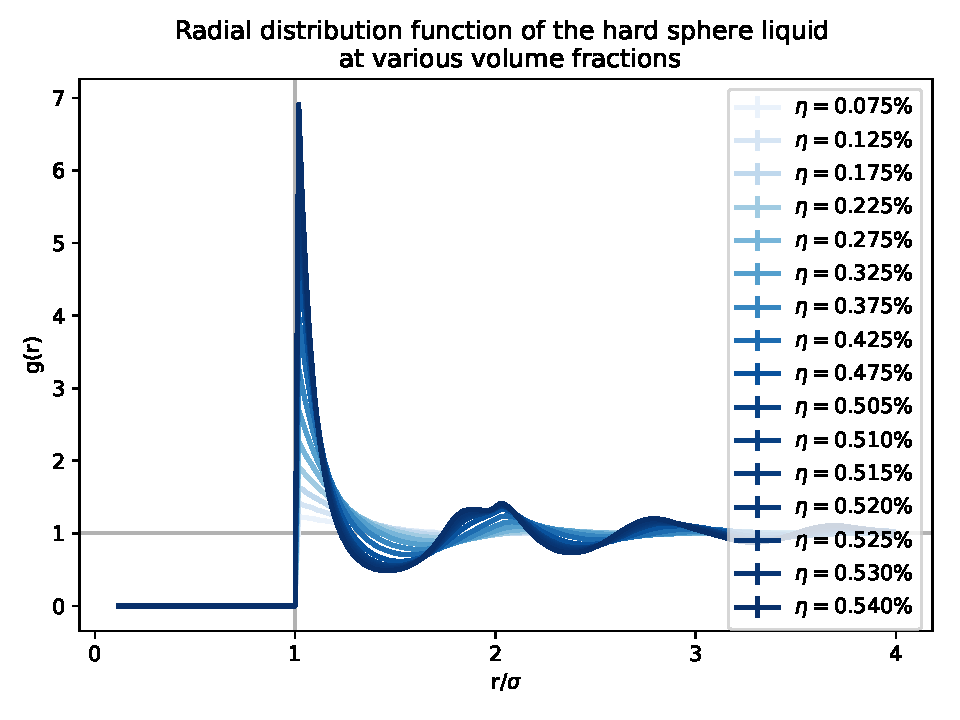
\includegraphics[width=0.7 \linewidth]{RDF.pdf}
\caption{Radial distribution functions for a range of volume fractions. The colouring corresponds to the used volume fraction.}
\label{fig:rdf_overview}
\end{figure}

To compare with Percus-Yevick approximation the radial distirbution function for two single volume fractions is shown with the corresponding theoretical solution in \autoref{fig:rdf_py}.
\begin{figure}[h]
\centering
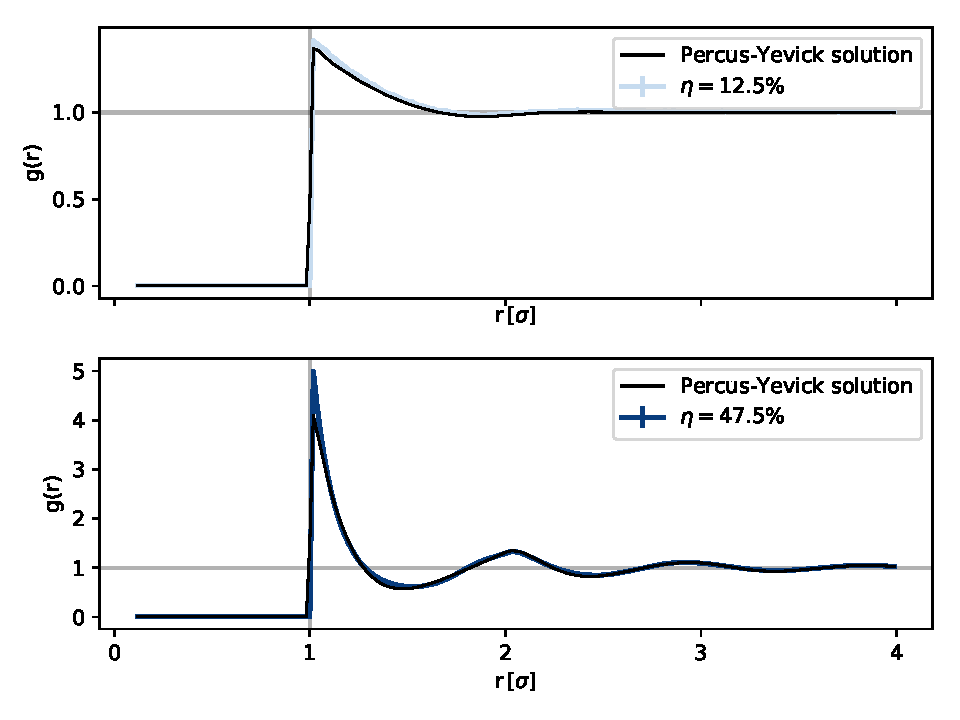
\includegraphics[width=0.7 \linewidth]{RDF_percus_yevick.pdf}
\caption{Radial distribution function for the hard sphere system at a low and at a high volume fraction of the liquid together with the theoretical prediction from the Percus-Yevick approximation.}
\label{fig:rdf_py}
\end{figure}

As highlighted for example in \cite{Hansen2006} the theoretical approximation has some flaws as can be seen with $g(r)|_{r=1\sigma}$ being too low for the Percus-Yevick approximation. Eventhough we see that overall the two radial distribution functions follow each other rather closely.\\
Such we are confident that the elaborated simulation code is capable of producing accurate data in other contexts as well.\\

\todo{It seems in the hansen and mcdonal that the peak below 2 sigma is also not present in their MC g(r), is there a reason for this?}

\section{Estimate of required resources}
\label{sec:resources}
To choose system parameters senseful calculation times and file sizes of the simulation were characterized. This was of interest as the program was supposed to run on the NEMO high performance computing cluster which puts hard boundaries on calculation times which when treepassed can cause tremendous loss of data if not corretly caught by the program.\\
 
\subsection{Calculation time estimates}
\label{sec:calc_times}
The calculation time of the program was tested for a large range of different system sizes up to almost 9 million particles in the fluid state. As can be seen in \autoref{fig:calc_time} the calculation time increases proportional to the system size for the execution of a step as well as for a measurement of the fluid system. The calculation cost being of $\mathcal{O}(N)$ enables the study of large systems. Furthermore from the slope an expectation for the execution time of a single event can be deduced, as well as an expectation for the time necessary for a measurement. As discussed on the example of \autoref{fig:calc_q6q6} the dependence of the measurement routines on the largest cluster size were not seen here, as possile clusters remained rather small during these simulation times.\\

\begin{figure}[h!]
\centering
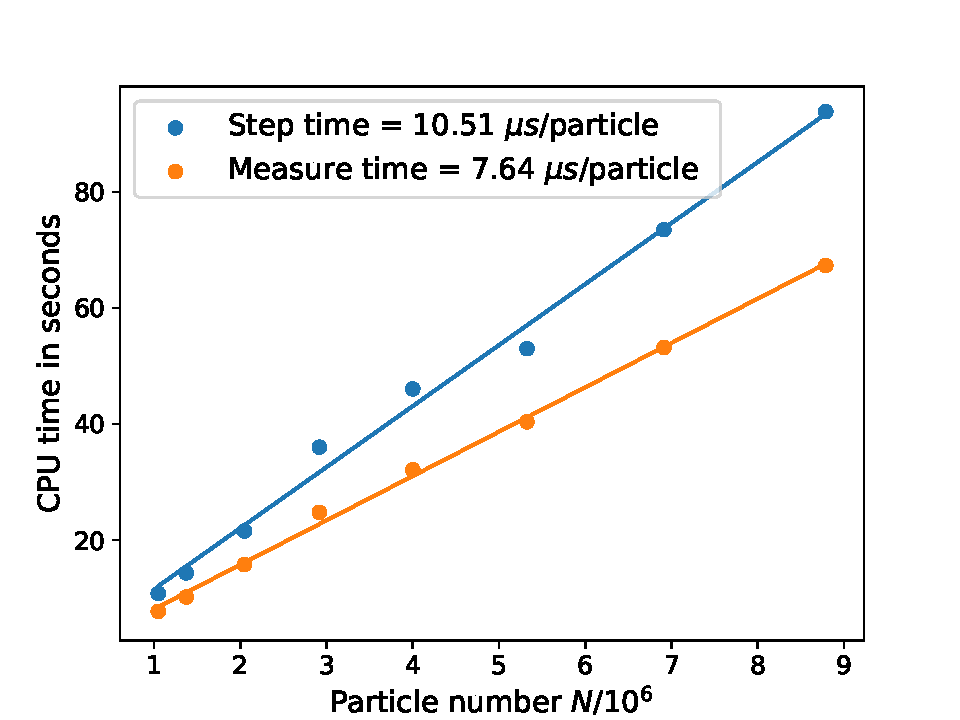
\includegraphics[width=0.7 \linewidth]{Calculation_times_measurement.pdf}
\caption{Overview of CPU time required for calculating a simulation step, consisting of an event for each particle, and a measurement of relevant quantities for the system. As assumed for a simulation algorithm with $\mathcal{O}(N)$ calculation effort, the data points can be described by a line rather well. As the CPU time is clearly related to the further workload of the CPU during the calculation it is also expected to find fluctuations if the other workload of the machine is not strictly controlled.}
\label{fig:calc_time}
\end{figure}


%Execution times for single steps have also been resolved with their distributions at 

%\begin{figure}[h!]
%\centering
%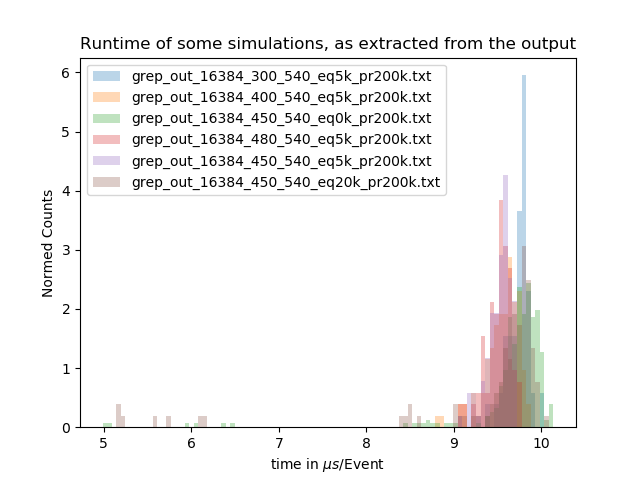
\includegraphics[width=0.7 \linewidth]{Simulation_runtimes.png}
%\caption{Histogram of CPU time required per execution of one event at different volume fractions. A small variation in the execution time is visible but the dependence is only small over a large range of volume fractions. Somewhat surprising are the outliers at about half the median calculation times for which no direct explanation could be found, except that mayhap the calculation node they were executed on did not have any further workload present at the time of execution.}
%\end{figure}
The effect of larger clusters was only investigated after problems with the runtime of the programs were traced back to these. The q6q6-order parameter routine was tested for larger clusters in a nucleating simulation with about 1 million particles within the box. As can be seen in \autoref{fig:calc_q6q6} the calculation cost of the cluster finding routine can be described with a quadratic dependence on the largest cluster. For an impression what this means we can use the calculation costs of a simulation step from \autoref{fig:calc_time} being about $t_{step} \approx \SI{10}{\mu s \per \text{particle} }$. Such the execution of one step takes about $\SI{10}{s}$ for 1 million particles. If a measurement is performed every 10th step, the calculation cost of the measurements without a large cluster remain below 10\%. But as the largest cluster grows to a few hundred thousand particles in size, the measurements can make up 30 \% and more of the calculation cost, or for a fixed number of steps, increase the calculation time by about 50 \%. This previously unseen effect lead to actual data loss as the combination of NEMO cluster policy and EDMD simulation program did not result in a save shutdown of the program after breaching the walltime limit of the NEMO cluster.\\

\begin{figure}[h!]
\centering
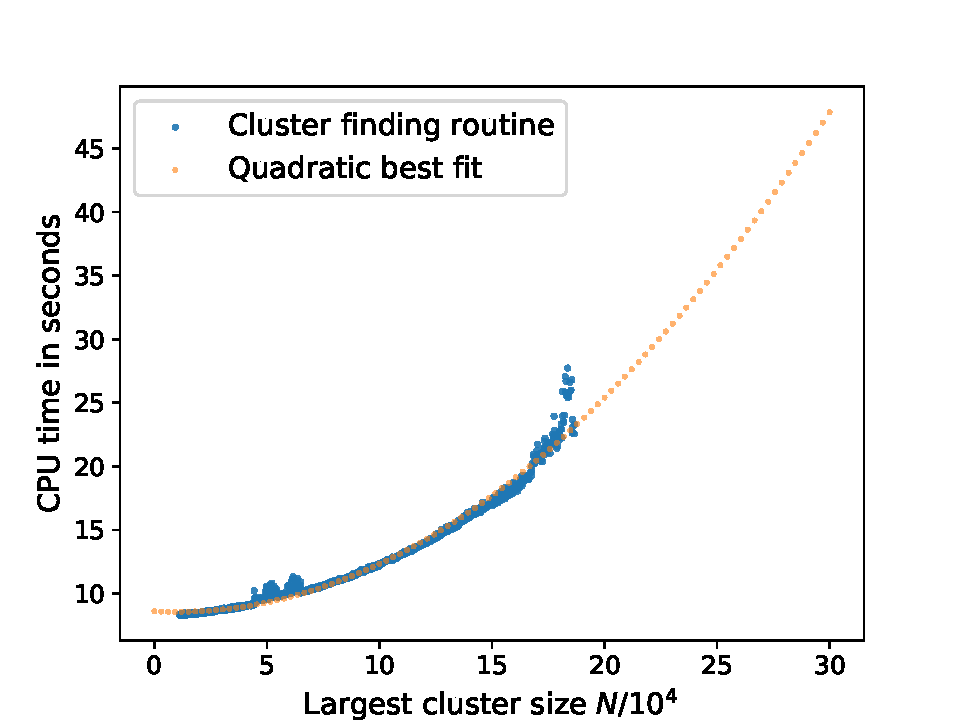
\includegraphics[width=0.7 \linewidth]{q6q6_calculation_time.pdf}
\caption{Calculation time of the q6q6 order parameter at an increasing largest cluster size during one nucleation, together with the quadratic best fit indicating that the q6q6 routine calculation effort can be approximated by $\mathcal{O}({N_{lc}}^2)$ where $N_{lc}$ is the size of the largest cluster.}
\label{fig:calc_q6q6}
\end{figure}


\subsection{File sizes estimates}
\label{sec:file_size}
A further important constraint for the simulations are the produced amount of data. To get an impression of the filesizes, the required memory for snapshots, reset steps and other measurements were measured prior to the actual simulations. The results for a single snapshot containing all positions and velocities of all particles as well as the size of a single simulation reset step containing all positions, velocities, the FEL, all PEL's and all delayed times is shown in \autoref{fig:file_size}. It can be seen that the file size is directly proportional to the system size which clearly expected as each particle adds a further set of positions, velocities etc. to the saved data.\\
The memory costs of other measurements have been left out of \autoref{fig:file_size} as these only amount to substantial filesizes if measurements at about each step for long simulations are done.\\  

\begin{figure}[h!]
\centering
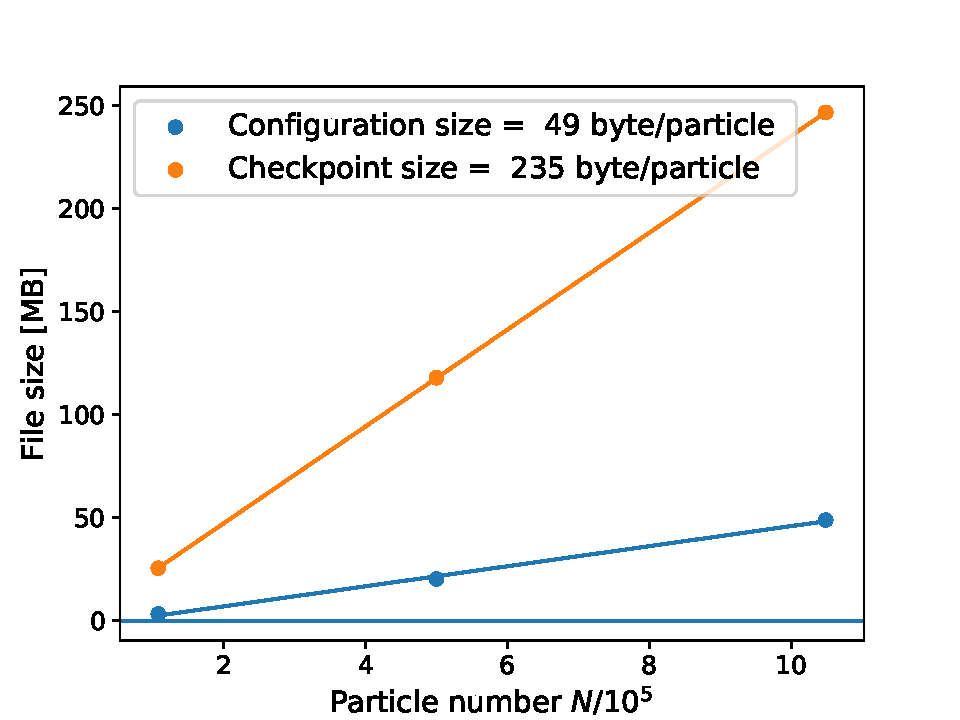
\includegraphics[width=0.7 \linewidth]{File_size.pdf}
\caption{Overview of filesizes when a single setup on the one hand and a single full simulation on the other hand is saved for comparison reasons together with their corresponding linear regression. while the linear regression for 3 points is statistically not exceedingly senseful it still remains a useful tool to extract the slope which corresponds to the required memory per particle and snapshot or reset simulation.}
\label{fig:file_size}
\end{figure}




\section{First produced data}
\label{sec:data}
The motivation for the simulation code is based on the interest in nucleation rates of the hard sphere system at varying volume fractions. To observe a nucleation the volume fraction of hard spheres has to be changed rapidly from lower ones where the system is in the stable fluid phase to higher ones where a meta stable fluid-solid phase exists. If this metastable phase is evolved in time nucleations can be observed as stochastic distributed events. To measure those without effects originating from the handling of the simulation, some parameters were tested within reasonable ranges prior to the data production.\\
For this simulation the equilibration steps as well as the inital density before the volume quench seemed like they could introduce unwanted artefacts, and thus we performed some smaller data series to evaluate if and when these effects might come into play.\\

The used test system is characterized by the figures in \autoref{tab:system_start_parameter_test}.

\begin{table}
\centering
\begin{tabular}{c|c}
Parameter & Value \\ \hline
N & 16384 \\
eq\_steps/particle & 100 ... 20000 \\
$\eta_i$ & 5\% ... 49 \% \\
$\eta_f$ & 54 \% \\
\end{tabular}
\caption{Input parameters of test systems probing the dependence on equilibration steps and inital density.}
\label{tab:system_start_parameter_test}
\end{table}

The general behaviour of the systems is analysed by inspecting the cluster distribution over time. The mean cluster distribution is shown in \autoref{fig:pnt_mean} together with the same data smoothed by a gaussian filter matrix. The smoothing is used because in a next step the difference between the mean cluster distribution and the cluster distributions with varying simulation parameters is compared, and without smoothing at low count rates only fluctuations are visible.\\


\begin{figure}[h!]
\centering
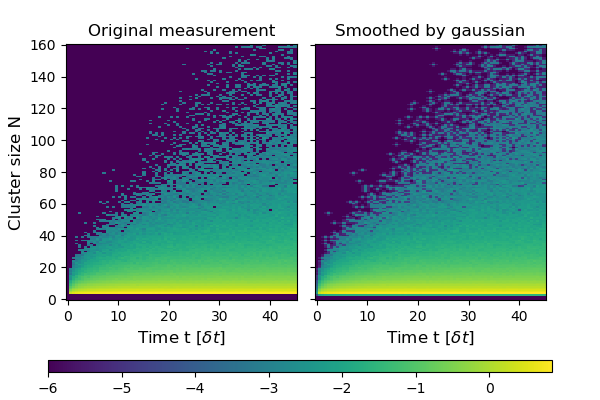
\includegraphics[width=0.7 \linewidth]{mean_pnt.png}
\caption{Heat map of the mean cluster distribution over time. The diagram encompasses 800 trajectories of 16384 particles each. The colouring indicates the logarithm of the mean cluster occurance corresponding to a probability in the stationary case.}
\label{fig:pnt_mean}
\end{figure}

From \autoref{fig:pnt_mean} we can see how the system behaves after a volume quench into the metastable region. In the liquid rarely any clusters are present and thus directly after the quench no clusters are present either as the spatial configuration requires time to rearange into clusters. In the later evolution we see how clusters form, and soon after begin to nucleate leaving the range of the diagram.\\

To compare simulations with varying parameters the quantity defined in \autoref{eqn:pnt_delta} is used, where complications with zero values are circumvented by fixing these values below the regular signal.\\ Three samples of this comparison are shown in \autoref{fig:pnt_eq_step_comparison} and \autoref{fig:pnt_eq_step_comparison}. The colouring indicates $\Delta_{p(N,t)}$ defined in \autoref{eqn:pnt_delta}. As mentioned above the quantities $p_i(N,t)$ and $\langle p(N,t) \rangle$ have been smoothed by a gaussian filter, because the number of samples included, with 100 trajectories per series, were not sufficent to produce smooth distributions at the given sampling rate. Such without smoothing only fluctuations would be visible.\\ 

\begin{align}
\label{eqn:pnt_delta}
\Delta_{p(N,t)} = log ( | \frac{p_i(N,t)}{\langle p(N,t) \rangle} -1 | )
\end{align}

\begin{figure}[h!]
\centering
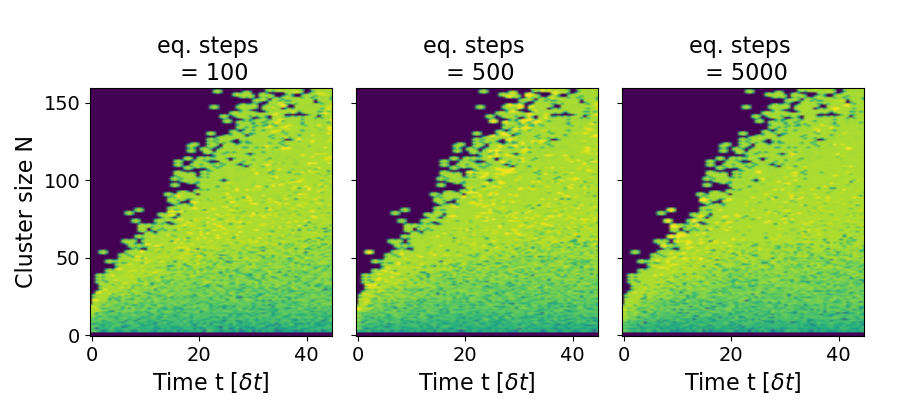
\includegraphics[width=0.7 \linewidth]{pnt_comparison_eq_steps.png}
\caption{Heat map of differences between the cluster distributions within simulations carried out with varying the length of the equilibration phase. The quantity used for colouring is defined in \autoref{eqn:pnt_delta}, where yellow indicates a large difference while blue indicates a small difference. Providing a legend of the colouring is ommited as $\Delta_{p(N,t)}$ has no further use as to indicate differences and actual values do not add any use.}
\label{fig:pnt_eq_step_comparison}
\end{figure}


\begin{figure}[h!]
\centering
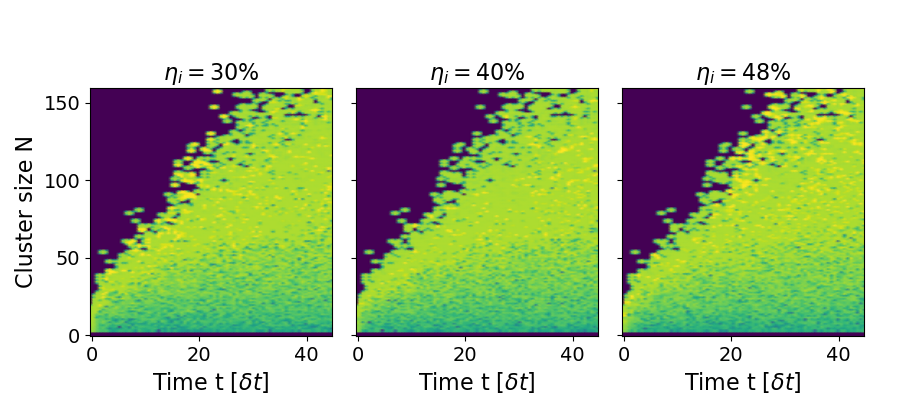
\includegraphics[width=0.7 \linewidth]{pnt_comparison_rho.png}
\caption{Heat map of differences between the cluster distributions within simulations carried out with varying the volume fraction of the liquid during the equilibration phase. The quantity used for colouring is defined in \autoref{eqn:pnt_delta}, where yellow indicates a large difference while blue indicates a small difference. Providing a legend of the colouring is ommited as $\Delta_{p(N,t)}$ has no further use as to indicate differences and actual values do not add any use.}
\label{fig:pnt_rho_comparison}
\end{figure}

On first sight none of them differ in their general behaviour. Because at t=0 after the quench no clusters have formed yet and also no clusters were present in the stable liquid, the difference between all simulations is zero, indicated by the blue region in the top left corner. The features visible on the edge between the zero region and the nonzero region on the other side are the same, because they are features of the mean distribution carried through. Actual differences not due to fluctuations can only be seend within the green and yellow non-zero region, but none such differences is observed.\\

While it seems like the inital volume fraction of $\eta=0.4$ and $eq\_steps = 5000$ include less irregular fluctuations, dramatic effects from choosing the simulation parameters can be excluded. Intresting in this context are esspecially the simulations with $eq\_steps = 100$ because after executing 100 events/particle on average, the inital perfect crystal configuration is only on the verge of not being detected anymore. Such one could expect that these configurations might be stoill close to crystalization, but instead we do not detect any significant difference.\\

A further more quantifying analysis of the differences is given by calculating the mean nucleation rates assuming classical nucleation theory. This is done for the data shown in \autoref{fig:comparison_nucleation_rates}. The calculations of the rates have been carried out as described in \autoref{sec:induction_times}.

\begin{figure}[h!]
\centering
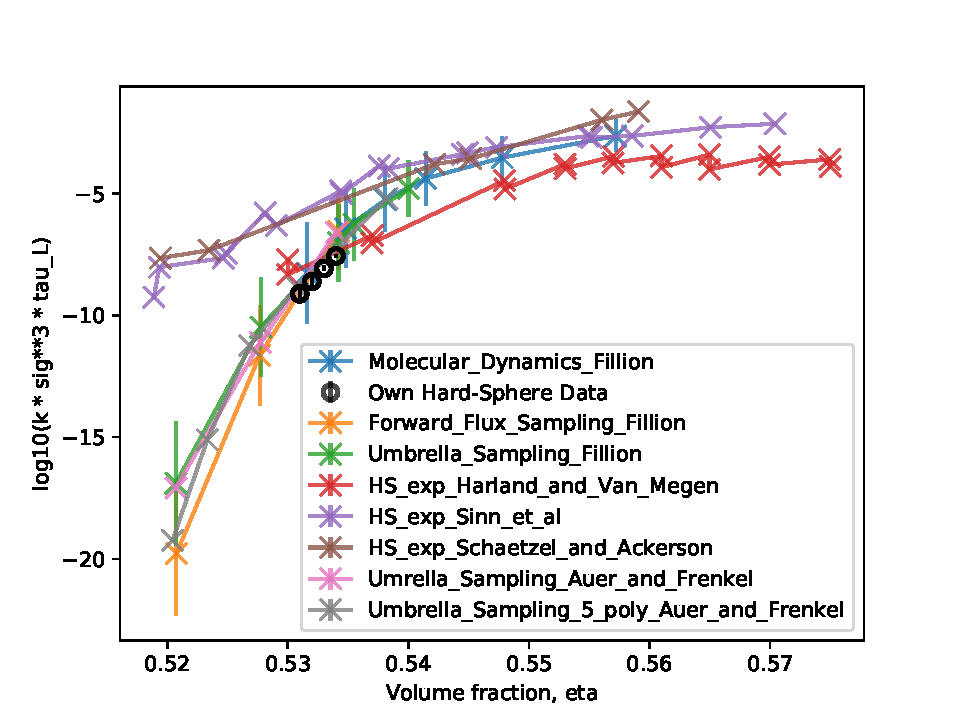
\includegraphics[width=0.7 \linewidth]{nucleation_rate_comparison.pdf}
\caption{Comparsion of nucleation rates under CNT assumptions for different inital densities during equilibration with eq\_steps fixed at 5000, as well as varying eq\_steps with $\eta_i$ fixed at 0.45. }
\label{fig:comparison_nucleation_rates}
\end{figure}

As we see no significant difference in the nucleation rates can be observed even for the bold setting of only 100 events per particle for the equilibration phase. Eventhough it can be seen that for this special case the rate is a little higher, but it may as well be a stochatic flucutaion.\\

Overall we conclude in this chapter that as long as parameters are set within reasonable boundaries, we expect not to have systematic influences of simulation parameters. 


%\Floatbarrier

\section{Possible extensions}
\label{sec:simulation_ext}
The program at this state is capable of simulating large systems including compression and relaxation. Extensions can aim at either increasing complexity or size of the systems. 

\subsection{Varying radius}
\label{sec:extension_radius}
A further notch of complexity is to include polydispersity into the simulation. For this purpose the prediction of collisions has to be adjusted. When looking at the derivation of \autoref{eqn:collision_prediction} it is found that $\sigma$ being the former diameter of a sphere in the monodisperse case has to be changed to $\sigma=R_i+R_j$. In the equations the same defiitions of scalar products are used as before in \autoref{sec:EDMD}.

\begin{align}
\label{eqn:collision_prediction}
\Delta t &= \frac{(rr - \sigma^2 )}{ - rv + \sqrt{ (rv)^2  - vv (rr - \sigma^2 )}}
\end{align} 

For a physical model in which the particles are made of some matter with constant density the change of the radius is also accompanied by a change of the mass. This has to be taken into account when assigning the velocities after a collision as written in \autoref{eqn:var_mass}.

\begin{align}
\label{eqn:var_mass}
\vec{v}_i{\,'} = \vec{v}_i + \frac{2 m_j \; (rv)}{(m_i + m_j) \sigma^2} \cdot (\vec{r}_j - \vec{r}_i) \nonumber \\
\vec{v}_j{\,'} = \vec{v}_j + \frac{2 m_i \; (rv)}{(m_i + m_j) \sigma^2} \cdot (\vec{r}_j - \vec{r}_i)
\end{align}

A small caveat is given by the fact that the simulations should be run within the center of mass frame, as otherwise unnecessary transition events have to be calculated. The corresponding assignemnt of velocities works as follows.\todo{do the center of mass assignement}

\subsection{Muliprocessing}
\label{sec:extension_MP}
It further would be possible to precalculate different events on different processors, thereby speeding up simulations. This requires the execution of events not in the strict time order used for the EDMD algorithm shown before. Instead a check should be implemented to only execute events which are spatially seperated by some distance. This might make it possible to change only little of the dynamics. Eventhough a problem conserning this idea is that the simulation code would be required to consume less memory as this would be the bottleneck of the system sizes.\\
Such rather large changes would be necessary to impelemnt parrallel EDMD simulations. Either way it could help making system of about 100 million particles feasible.   


